\chapter{H$_{2}$O in an external electric dc field}
\label{ch:dc_h2o}

% H2O in strong dc fields
% effective potential
% outline of the chapter

The stark resonance parameters, which characterize the shift of the
molecular energy levels under an external dc field, are fundamental in
the study of the strong dc field ionization of molecular orbitals
(\textsc{mo}s). In the case of the water molecule, the multicentre
nature of the combined Coulomb interactions and, consequently, the
additional degrees of freedom, make the strong dc field ionization of
H$_{2}$O an attractive and challenging problem from the point of view
of a theoretical description as well as experimentally. Complex
variable techniques, such as an exterior complex
scaling~\cite{Simon_1979,ecsScrinzi} and complex-absorbing
potentials~\cite{RissMeyer_1993,Krause_2014}, have been implemented in
order to address the problem of molecular static-field ionization and
compute the induced Stark resonances.

The dc Stark problem for the H$_{2}$O valence orbitals is addressed in
this chapter by the implementation of a modified exterior complex
scaling approach that allows to study the ionization of the molecular
orbitals of H$_{2}$O under a strong dc field. The construction of an
effective potential, which reflects the indivual properties of the
orbitals, is crucial in this analysis. In Sec.~\ref{ch:h2o_structure},
we formulate the problem with emphasis on the representation of the
molecular orbitals. The exterior complex scaling formalism is
introduced in Secs.~\ref{ch:1b1_1b2} and~\ref{ch:3a1} as a crucial
step in finding a numerical solution to a spherically symmetric
problem, in the case of the $1b_{1}$ and $1b_{2}$ orbitals, and the
problem of a non-central effective potential, in the case of the
$3a_{1}$ orbital. The Stark resonance parameters are then presented in
Sec.~\ref{ch:stark_params}, in which the symmetry properties of the
orbitals are considered independently. The analysis presented in this
chapter compiles that of~\cite{sarias_2016,sarias_2017}.


\section{Molecular orbital representation of H$_{2}$O}
\label{ch:h2o_structure}
% Formulation of the Problem

The starting point for this study is the Hartree-Fock (\textsc{hf})
calculation of the H$_{2}$O molecular states using a single-center
Slater orbital
basis~\cite{Moccia_1964,Moccia_JCP_2164,Moccia_JCP_2176}, applied to
collision studies~\cite{Montanari_2013} and compared to experimental
electron spectroscopy~\cite{Hafied_2007}. Other elaborate descriptions
of the molecular structure of H$_{2}$O formulated within the
independent-electron approximation by the self-consistent field
(\textsc{scf}), or variational Hartree-Fock method with multicentre
Slater orbitals, in which the pioneering work of Ellison and
Shull~\cite{EllisonShullh2o_1955} is revised, are reference for
describing the electronic structure of diatomic molecules by means of
an expansion of Slater
orbitals~\cite{Pitzer_1968,Pitzer_1970}. However, the direct
application of these multicentre orbitals for strong-field studies
implies significant computational and methodological challenges.

The present work is intended to study the valence molecular orbitals
of H$_{2}$O, $1b_{1}$, $1b_{2}$ and $3a_{1}$. The wavefunctions for
the $1b_{1}$ and $1b_{2}$ molecular orbitals, which correspond to the
$2p_{x}$ and $2p_{y}$ oxygen orbitals, are dominated by a single
angular mometum symmetry. The $3a_{1}$ \textsc{mo}, on the other hand,
consists mainly of the oxygen $2s$ and $2p_{z}$ and the hydrogen $1s$
atomic orbitals.

The general expression for the basis functions, introduced as a set of
single-center
wavefunctions~\cite{Moccia_1964,Moccia_JCP_2164,Moccia_JCP_2176}, is
defined as a Slater-type orbital (\textsc{sto}),
%
\begin{eqnarray}
  \begin{split}
 f_{nlm}(\zeta,r,\theta,\phi) & = & \sqrt{\frac{(2\zeta)^{2n+1}}{(2n)!}}
 r^{n-1} \exp(-\zeta r) S_{l, m}(\theta,\phi),
 \end{split}
\label{eq:sto}
\end{eqnarray}
%
where the angular part $S_{l,m}(\theta,\phi)$ represents real
spherical harmonics. The expansion coefficients and nonlinear
coeficients $\{\zeta_{i}\}$, determined by the Roothaan's
self-consistent-field method~\cite{Moccia_1964,Roothaan_1951}, are
used to construct a reduced form of the radial functions that describe
all the molecular orbitals. More specifically, we are interested in
using a reduced \textsc{sto} expansion to construct an effective
pontential that describes the response of the H$_{2}$O valence
orbitals when applying an electric dc field along the symmetry axis
(i.e., the $z-$axis).

Based on their symmetry properties, independent descriptions of the
valence molecular orbitals of H$_{2}$O are constructed. The dominant
components of the $1b_{1}$ and $1b_{2}$ orbitals, namely the $np_{x}$
and $np_{y}$ parts, are used to derive spherically symmetric effective
orbital-dependent potentials~\cite{sarias_2016}. While a similar
procedure is implemented for the $3a_{1}$ orbital, i.e., retaining the
$np_{z}$ parts of the \textsc{mo}, the strong asymmetry introduced by
the two protons located in the $y-z$ plane leading to significant
admixtures of $s-$type Slater orbitals in the Moccia
\textsc{sto}s~\cite{Moccia_1964} would have been ignored with a
spherically symmetric potential. Hence, for the dc ionization problem
of the $3a_{1}$ \textsc{mo}, \textsc{sto}s of type $2s$ and $2p_{z}$
are incorporated in the analysis.


% representation of the orbitals, fig.1 in the papers (also fig.2 of
% the jphysb), with related comments

\section{$1b_{1}$ and $1b_{2}$ molecular orbitals}
\label{ch:1b1_1b2}

The Schr\"{o}dinger equation for the bound-state problem of a
molecular orbital within an effective potential $V_{\mathrm{eff}}(r)$
is expressed in shperical polar coordinates as
%
\begin{eqnarray}
  [ -\frac{1}{2} \frac{d^2}{dr^2} + \frac{\hat{L}^2}{2r^2} + V_{\rm{eff}}(r)] \psi
  & = & E\psi,
\label{eq:sch_noCS}
\end{eqnarray}
%
where $\hat{L}^{2}$ is the orbital quantum momentum operator. The
present study involves the construction of the effective
orbital-dependent potential $V_{\mathrm{eff}}(r)$ extracted from the
single-centre Moccia wave functions~\cite{Moccia_1964}. Then an
exterior complex scaling (\textsc{ecs})~\cite{Simon_1979} is applied
to determine the numerical solution of the problem associated with a
molecular orbital in the presence of a strong electric dc field
applied along the $\hat{z}-$direction~\cite{sarias_2016}. A schematic
representation of the geometry of the system is shown in
Figure~\ref{fig:h2o_1b1_1b2}, where the orientation of the $1b_{1}$
and $1b_{2}$ \textsc{mo}s is indicated with respect to the plane where
the protons are located. The direction of the applied electric field
along $\hat{z}$ is included as well.

\begin{figure}
  \centering
  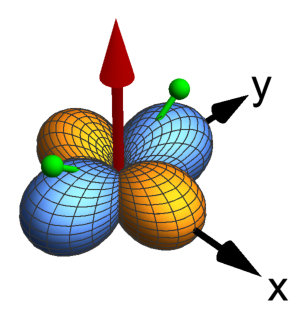
\includegraphics[width=0.25\textwidth]{figures/ch_H2O/1b1_1b2/orbitals.eps}
  \caption{Schematic display of the $1b_{1}\approx 2p_{x}$ (shown in
    yellow along the $x$ axis) and $1b_{2}\approx 2p_{y}$ (shown in
    blue along the $y$ axis) molecular orbitals. Also indicated (in
    green on the $y-z$ plane) is the orientation of the protons. The
    $z$ axis (in red) is the direction of the external electric field
    of strength $F_{0}$.}
  \label{fig:h2o_1b1_1b2}
\end{figure}


As a first step in solving Eq.~(\ref{eq:sch_noCS}) for the H$_{2}$O
molecular orbitals, we introduce the reduced single-centre Moccia
wavefunction,
%
\begin{eqnarray}
  \begin{split}
    \psi_{1b_{1},1b_{2}}(r) & = & \sum\limits_{i} c_{nlm} f_{nlm}(\zeta_{i}, r),
    \label{eq:sto_1b1_1b2}
  \end{split}
\end{eqnarray}
%
which approximates the molecular orbital by an eigenstate of a
spherically symmetric potential. The functions $f_{nlm}(\zeta_{i},r)$
represent the radial part of the Slater orbitals~(\ref{eq:sto}) with
$|m|=1$ for the magnetic quantum number, in which the \textsc{sto}
expansion is limited to $2p_{x}$ and $2p_{y}$ orbitals,
respectively. The set of expansion coefficients and non-linear
coefficients in~(\ref{eq:sto_1b1_1b2}), given in
Table~\ref{tab:1b11b2_coef}, represents a reduced selection of the
expansion parameters given by Moccia for the ground state of the water
molecule~\cite{Moccia_1964}.

\begin{table}[t]
 \centering
  \caption{\label{tab:1b11b2_coef} Expansion coefficients and
    nonlinear coefficients for the $1b_{1}$ and $1b_{2}$ molecular
    orbitals of H$_{2}$O. The parameters used in our reduced
    \textsc{sto} expansion are indicated as included.}
  \begin{tabular}{lrrrr}
    \toprule
    $(n,l, m)$ & & $\zeta_{i}$ & $c_{nlm}^{1b_{1}}$ & $c_{nlm}^{1b_{2}}$ \\
    \midrule
    $(2,1,1)$ & included & $1.510$ & $0.72081$ & --~~ \\
    $(2,1,1)$ & included & $2.440$ & $0.11532$ & --~~ \\
    $(2,1,1)$ & included & $3.920$ & $0.24859$ & --~~ \\
    $(3,2,1)$ & excluded & $1.600$ & $0.05473$ & --~~ \\
    $(3,2,1)$ & excluded & $2.400$ & $0.00403$ & --~~ \\
    $(4,3,1)$ & excluded & $1.950$ & $0.00935$ & --~~ \\
    $(4,3,3)$ & excluded & $1.950$ & $-0.02691$ & --~~ \\
    $(2,1,-1)$ & included & $1.510$ & --~~ & $0.88270$ \\
    $(2,1,-1)$ & included & $2.440$ & --~~ & $-0.07083$ \\
    $(2,1,-1)$ & included & $3.920$ & --~~ & $0.23189$ \\
    $(3,2,-1)$ & excluded & $1.600$ & --~~ & $0.25445$ \\
    $(3,2,-1)$ & excluded & $2.400$ & --~~ & $-0.01985$ \\
    $(4,3,-1)$ & excluded & $1.950$ & --~~ & $0.04526$ \\
    $(4,3,-3)$ & excluded & $1.950$ & --~~ & $-0.06381$ \\
    \bottomrule
  \end{tabular}
\end{table}

In order to determine the effective potential corresponding to each
molecular orbital, the wavefunction~(\ref{eq:sto_1b1_1b2}) is inserted
into the single-electron Schr\"{o}dinger equation~(\ref{eq:sch_noCS}),
which is then solved for $V_{\mathrm{eff}}^{(1)}(r)$. Afterwards, the
so-called Latter correction~\cite{LatterCor_1955,sarias_2016} is
applied to ensure that the effective potential converges
asymptotically to $-1/r$, as expected in a Coulomb potential:
%
\begin{eqnarray}
V_{\mathrm{eff}}(r) = \left\{
\begin{split}
V_{\mathrm{eff}}^{(1)}(r)\  & \mathrm{for} & r < r_{0} \\
-1/r\  & \mathrm{for} & r > r_{0}
\end{split}
\right.
,
\label{eq:coulomb_tail}
\end{eqnarray}
%
where the point $r_{0}$ is determined from $V_{\mathrm{eff}}^{(1)}(r_{0}) =
-1/r_{0}$, and is found to be sufficiently large that the original
self-consistent field orbital energy used to derive
$V_{\mathrm{eff}}^{(1)}(r)$ is close to the eigenenergy
of~(\ref{eq:sch_noCS}), with at least two significant digits of
agreement, with $V_{\mathrm{eff}}(r)$ given
by~(\ref{eq:coulomb_tail}).

\begin{figure}
  \centering
  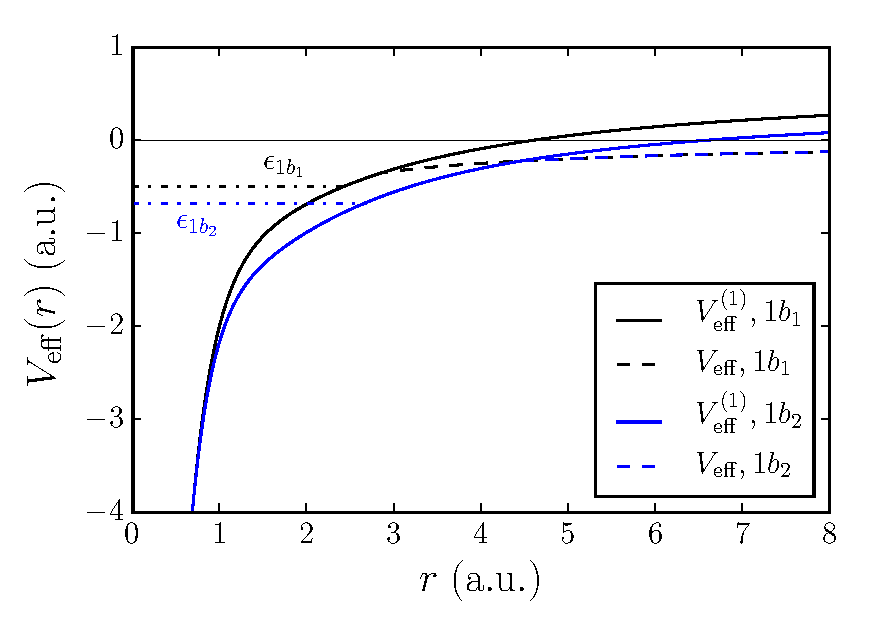
\includegraphics[width=0.75\textwidth]{figures/ch_H2O/1b1_1b2/Veff1b11b2.eps}
  \caption{Electronic effective potential in atomic units for the
    $1b_{1}\approx 2p_{x}$ (black) and $1b_{2}\approx 2p_{y}$ (blue)
    \textsc{mo}s of the H$_{2}$O molecule. The solid lines give the
    potential as derived from~(\ref{eq:sch_noCS}) using the
    \textsc{scf} orbitals and eigenenergies, while the dashed lines
    show the potentials after the Latter correction is applied. The
    dot-dashed lines indicate the eigenenergies obtained from the
    Moccia wavefunctions~\cite{Moccia_1964}.}
  \label{fig:Veff1b11b2}
\end{figure}

Figure~\ref{fig:Veff1b11b2} shows a comparison of the effective
potential $V_{\mathrm{eff}}^{(1)}(r)$ (solid lines), with black
representing the $1b_{1}$ \textsc{mo} and blue representing the
$1b_{2}$ \textsc{mo}, derived from the Moccia wavefunctions
representing the $1b_{1}$ and $1b_{2}$
\textsc{mo}s~\cite{Moccia_1964}, and the transformed electronic
potential $V_{\mathrm{eff}}(r)$ (dashed lines) after the Latter
correction was implemented. The effective potentials for the $1b_{1}$
and $1b_{2}$ \textsc{mo}s are given as the shallower and deeper
curves. As Figure~\ref{fig:Veff1b11b2} illustrates, one drawback of
the method is that the effective potential is orbital dependent. A
direct consequence is that the value of $r=r_{0}$, which sets the
position in $r$ where the Coulombic tail is imposed, differs between
the \textsc{mo}s, being almost two times larger for the $1b_{2}$
compared to the $1b_{1}$ \textsc{mo}.


\subsection{PDE approach and exterior complex scaling}
\label{ch:ecs_1b11b2}

This section discusses further the formalism implemented to calculate
the relevant resonance parameters in the problem of the H$_{2}$O
molecule exposed to a strong dc field. Having obtained an effective
potential to define the field-free Schr\"{o}dinger
equation~(\ref{eq:sch_noCS}) for an orbital obtained in the
\textsc{scf} method~\cite{Moccia_1964}, we proceed with the problem of
the molecule ionized by a strong dc field.

When an electric field is applied in the $\hat{z}$ direction,
$\mathbf{F} = F_{0}\hat{z}$, the separation of variables ansatz as
applied to the Schr\"{o}dinger equation~(\ref{eq:sch_noCS})
%
\begin{eqnarray}
  \begin{split}
    \psi(r,\theta,\phi) & = & \psi(r,\theta)\exp(im\phi)
  \end{split}
\label{eq:sov}
\end{eqnarray}
%
leads to a partial differential equation (\textsc{pde}) in spherical
coordinates that represents the Stark problem for an H$_{2}$O orbital:
%
\begin{eqnarray}
 \begin{split}
  -\frac{1}{2} \frac{\partial^{2}\psi}{\partial r^2} - \frac{1}{2r^2}
  (\frac{\cos\theta}{\sin\theta} \frac{\partial\psi}{\partial\theta} + 
  \frac{\partial^2\psi}{\partial\theta^2})
  + (\frac{m^2}{2r^2 \sin^2\theta} + V_{\mathrm{eff}}(r) - E +
  F_{0}r\cos\theta)\psi & = & 0.
  \end{split}
\label{eq:pde}
\end{eqnarray}
%
Here the complex eigenenergy $E$ contains the information about the
resonance position (real part), i.e., $E_{R}$ and width $\Gamma$
(imaginary part is $-\Gamma/2$), and may be expressed as
%
\begin{eqnarray}
E & = & E_{R} + iE_{I} = E_{R} - i\frac{\Gamma}{2}.
\label{eq:complex_E}
\end{eqnarray}
%
The imaginary part $\Gamma$ is related to the lifetime of the decaying
state $\tau$ via $\Gamma\tau = 1$. For the $1b_{1}$ and $1b_{2}$
orbitals we have $m=\pm 1$, respectively. The presence of the
effective potential $V_{\mathrm{eff}}(r)$ makes this problem
challenging in the sense that it is not possible to obtain separable
solutions like for the hydrogen atom in which a pure Coulomb potential
leads to separability in parabolic coordinates, as was discussed
in~\cite{Telnov_1989}. It is then necessary to generate a more general
solution by solving the \textsc{pde} numerically, e.g., by applying a
finite-element method.

The ionization regime of the water molecule is described by means of a
non-Hermitian Hamiltonian that reveals discrete resonance eigenvalues
containing information about the quasibound states that tunnel through
the barrier or escape over the potential barrier for strong
fields. Among the different techniques implemented in the study of
atomic resonances, a standard tool is the method of complex
scaling~\cite{complexScaling,complexScalingBaslev,complexScalingSimon}. This
approach consists in extending the analytic domain of the Hamiltonian
of a given system by means of a mapping operator that results in
complex eigenvalues which provide direct access to the resonant states
of the Stark problem. For most phenomenological potentials, such as
molecules with fixed internuclear distances, a modified method of
scaling is required as an extension to cases where the potential is
analytic only outside some bounded region. In these cases, the
approach of exterior complex scaling (\textsc{ecs})~\cite{Simon_1979}
is more appropriate, as the potential needs to have analyticity
properties only in the region affected by the scaling, where one can
look for solutions which decay exponentially in the assymptotic region
of the potential. Both methods have been widely used in scattering
problems~\cite{complexScalingBaslev, complexScalingSimon}, in studies
of the Stark problem for multi-electron
systems~\cite{ScrinziJChemPhys_ECS,ScrinziJPhysB_ECS}, as well as in
time-dependent Schr\"{o}dinger equation problems for strong
fields~\cite{ecsRuiz, ecsTao, ecsScrinzi}.

For our aim of studying the field ionization properties of H$_{2}$O
orbitals, we implement a modified \textsc{ecs} technique in which the
radial coordinates are extended into the complex plane by a phase
factor, which is turned on gradually beyond some distance from the
origin. This method allows us to address the tunneling and
over-barrier ionization problem by avoiding the complication of
describing quasibound states with outgoing waves for $r \to
\infty$. In the present work, the complex scaling transformation is
given by
%
\begin{eqnarray}
  \begin{split}
    r & \rightarrow & r\exp(i\chi(r)),
  \end{split}
\label{eq:ecs_r}
\end{eqnarray}
%
where $\chi$ is defined as a function of the $r$ coordinate with the
purpose of making the scaling gradually effective from some vicinity
of $r = r_{\mathrm{s}}$ on,
%
\begin{eqnarray}
  \begin{split}
    \chi(r) & = & \frac{\chi_{\mathrm{s}}}{1+\exp[-\frac{1}{\Delta r}
        (r - r_{\mathrm{s}})]}.
  \end{split}
\label{eq:ecs_theta}
\end{eqnarray} 
%
For given $r_{\mathrm{s}}$ one has to choose $\Delta r$ to be
sufficiently small, so that the function $\chi(r)$ starts from small
values at $r = 0$. For large $r$, it converges to the value
$\chi_{\mathrm{s}}$.

The set of possible values for the asymptotic scaling angle
$\chi_{\mathrm{s}}$ and the parameters $r_{\mathrm{s}}$ and $\Delta
r$, which control where and how quickly the scaling is turned on, is
explored in detail in order to establish how sensitive the
\textsc{pde} solutions are and to test the effectiveness of the
complex scaling technique to absorb the outgoing wave. Numerous tests
were carried out to ensure that the ``exact'' results of
Telnov~\cite{Telnov_1989} for atomic hydrogen orbitals including $2p$
are reproduced.

In order to investigate the effects of the dc field on the H$_{2}$O
orbital energies it is necessary to consider the extra terms that the
\textsc{ecs}~(\ref{eq:ecs_r}) introduces in the Schr\"{o}dinger
equation~(\ref{eq:pde}). Additionally, we need to turn the scaling on
only in the regime $r > r_{0}$, as Eq.~(\ref{eq:coulomb_tail})
indicates, such that we have a simple Coulomb potential in the scaling
region. In order to make use of standard finite-element methods, the
complex-valued wave function is separated into real and imaginary
parts, such that a system of coupled differential equations is
obtained as follows~\cite{sarias_2016}:
%
\begin{eqnarray}
  -\frac{1}{2}\frac{\partial^{2}\psi_{R}}{\partial r^2}-\frac{1}{2r^2}
  (\frac{\cos\theta}{\sin\theta}\frac{\partial\psi_{R}}{\partial\theta}+
  \frac{\partial^{2}\psi_{R}}{\partial\theta^2}) \nonumber\\
  +(\frac{m^2}{2r^2\sin^2\theta}+V_{\rm{eff}}^{R}(r)c_{2}-V_{\rm{eff}}^{I}(r)s_{2}
  -E_{R}c_{2}+E_{I}s_{2}+
  F_{0}r\cos\theta c_{3})\psi_{R} \nonumber\\
  +(-V_{\rm{eff}}^{R}(r)s_{2}-V_{\rm{eff}}^{I}(r)c_{2}+E_{R}s_{2}+E_{I}c_{2}-F_{0}r\cos\theta
  s_{3})\psi_{I} & = & 0, \nonumber\\
  \vspace{1cm}
  -\frac{1}{2}\frac{\partial^{2}\psi_{I}}{\partial r^2}-\frac{1}{2r^2}
  (\frac{\cos\theta}{\sin\theta}\frac{\partial\psi_{I}}{\partial\theta}+
  \frac{\partial^{2}\psi_{I}}{\partial\theta^2}) \nonumber\\
  +(\frac{m^2}{2r^2\sin^2\theta}+V_{\rm{eff}}^{R}(r)c_{2}-V_{\rm{eff}}^{I}(r)s_{2}
  -E_{R}c_{2}+E_{I}s_{2}+
  F_{0}r\cos\theta c_{3})\psi_{I} \nonumber\\
  +(V_{\rm{eff}}^{R}(r)s_{2}+V_{\rm{eff}}^{I}(r)c_{2}-E_{R}s_{2}-E_{I}c_{2}+F_{0}r\cos\theta
  s_{3})\psi_{R} & = & 0.
\label{eq:pde_system}
\end{eqnarray}
%
The labels $R$ and $I$ stand for real and imaginary parts,
respectively; also, the notation $[c_{k},s_{k}]$ is introduced to
represent $[\cos[k\chi(r)], \sin[k\chi(r)]]$, respectively, with
$k=2,3$ and $\chi(r)$ defined in~(\ref{eq:ecs_theta}). Note that the
effective potential has real and imaginary parts on account of the
coordinate transformation~(\ref{eq:ecs_r}).
 
The \textsc{pde} system~(\ref{eq:pde_system}) is solved numerically on
a rectangular mesh defined by the $(r, \theta)$ coordinates, which
take values in the domains $[\epsilon, r_{\mathrm{max}}]$ and
$[\eta,\pi - \eta]$, respectively. The parameters $\epsilon$ and
$\eta$ that define the coordinate ranges were chosen to be of the
order of $10^{-3}\ \mathrm{a.u.}$, and the $r$ coordinate extends to
$r_{\mathrm{max}} = 20\ \mathrm{a.u.}$ In order to find a correct set
of $\psi_{R{I}}(r,\theta)$ solutions, it is essential to impose proper
boundary conditions that ensure the wave functions vanish at the
limits of the mesh. For the $|m| = 1$ states we impose the condition
$\psi_{R{I}}(\epsilon,\theta) = \epsilon \sin(\theta) = \epsilon
P_{1}^{1}(\theta)$, which is consistent with the assumption that at
small $r = \epsilon$ the lowest term in an expansion in associated
Legendre polynomials dominates and behaves like $A r^{2}
\sin(\theta)$.

A two-parameter root search for $\{E_{R}, E_{I}\}$ is implemented by
solving the \textsc{pde} as if it were an inhomogeneous problem. We
pick a location in the $(r,\theta)$ plane where the probability
amplitude is expected to be large and vary $\{E_{R}, E_{I}\}$, i.e.,
effectively the complex energy $E$ to maximize the amplitude.


\section{$3a_{1}$ molecular orbital}
\label{ch:3a1}

% sec 2 of JPhysB
In this section we extend the approach to study the dc Stark problem
for the $3a_{1}$ molecular orbital of H$_{2}$O. Given the orientation
of this orbital with respect to the plane in which the two protons are
located it is deemed necessary to go beyond the spherical effective
potential approximation, which was implemented in
Sec.~\ref{ch:1b1_1b2} for the $1b_{1}$ and $1b_{2}$ orbitals, in order
to take into account the strong asymmetry introduced by the protons in
the $y-z$ plane and the significant admixtures of $s-$type Slater
orbitals in the \textsc{sto}s~\cite{Moccia_1964}.

The proposed method to address this problem is to define a reduced
single-centre Moccia wavefunction,
%
\begin{eqnarray}
\psi_{3a_{1}}(r,\theta) = \sum_{n,l} c_{nl0} \varphi_{nl0}(r,\theta).
\label{eq:3a1Moccia_expansion}
\end{eqnarray}
%
Here the $\varphi_{nl}(r,\theta)$ are Slater orbitals with $m=0$ for
the magnetic quantum number, and we limited the expansion to
\textsc{sto}s of $2s$ and $2p_{z}$ type. The parameters are given in
Table~\ref{tab:3a1_coef} and three $2p_{z}$ orbitals are mixed with
three $2s$-type orbitals. This set of coefficients represents a
reduced selection of the expansion parameters given by Moccia for the
ground state of the water molecule~\cite{Moccia_1964} also shown in
Table~\ref{tab:3a1_coef}.

\begin{table}[t]
\centering
\caption{\label{tab:3a1_coef} Expansion coefficients and non-linear
  coefficients for the $3a_{1}$ \textsc{mo}. The parameters used in
  our reduced \textsc{sto} expansion are indicated as included.}
\begin{tabular}{lrrr}
\toprule
$(n,l,m)$ & & $c_{nlm}$ & $\zeta_{i}$ \\
\midrule[0.25pt]
 $(1,0,0)$ & excluded & $-0.00848$ & $12.600$ \\
 $(1,0,0)$ & excluded & $0.08241$ & $7.450$ \\
\midrule[0.25pt]
 $(2,1,0)$ & included & $0.79979$ & $1.510$  \\
 $(2,1,0)$ & included & $0.00483$ & $2.440$  \\
 $(2,1,0)$ & included & $0.24413$ & $3.920$  \\
 $(2,0,0)$ & included & $-0.30752$ & $2.200$ \\
 $(2,0,0)$ & included & $-0.04132$ & $3.240$ \\
 $(2,0,0)$ & included & $0.14954$ & $1.280$ \\
\midrule[0.25pt]
 $(3,2,0)$ & excluded & $0.05935$ & $1.600$ \\
 $(3,2,0)$ & excluded & $0.00396$ & $2.400$ \\
 $(3,2,2)$ & excluded & $-0.09293$ & $1.600$ \\
 $(3,2,2)$ & excluded & $0.01706$ & $2.400$ \\
 $(4,3,0)$ & excluded & $-0.01929$ & $1.950$ \\
 $(4,3,2)$ & excluded & $-0.06593$ & $1.950$ \\
\bottomrule
\end{tabular}
\end{table}

The probability densities for the $3a_{1}$ orbital as obtained from
the reduced expansion~(\ref{eq:3a1Moccia_expansion}) and from the
Moccia self-consistent results are shown in
Figures~\ref{fig:3a1_reduced} and~\ref{fig:3a1_Moccia},
respectively. The protons (in red) lie in the $y-z$ plane. As
Fig.~\ref{fig:3a1_reduced} indicates, the contributions to the density
of the $2s-$type states reproduce the proper dependence of the
$3a_{1}$ probability density with the polar angle $\theta$, as the
broader hump is located on the negative $z-$axis in the same way as in
the complete Moccia representation shown in Fig.~\ref{fig:3a1_Moccia}.

\begin{figure}
  \centering
  \begin{subfigure}[b]{0.25\linewidth}
    \centering
    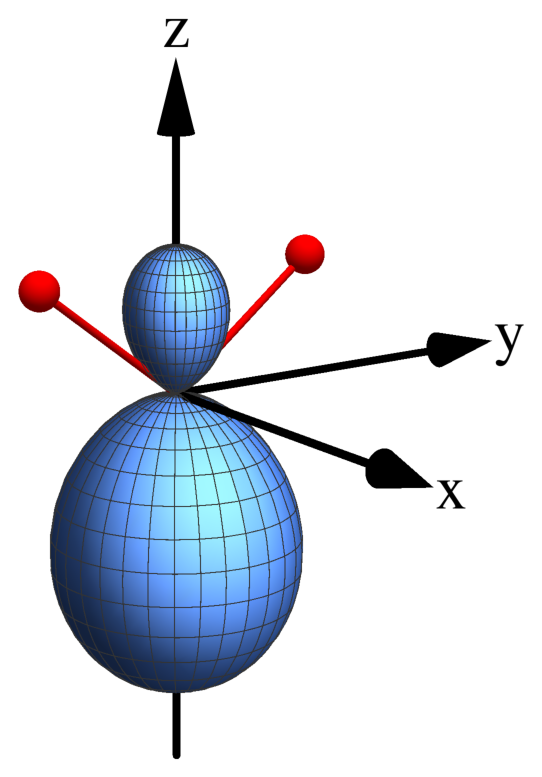
\includegraphics[width=\textwidth]{figures/ch_H2O/3a1/3a1extended.eps}
    \caption{Simplified $3a_{1}$ orbital}\label{fig:3a1_reduced}
  \end{subfigure}
  \,
  \begin{subfigure}[b]{0.25\linewidth}
    \centering
    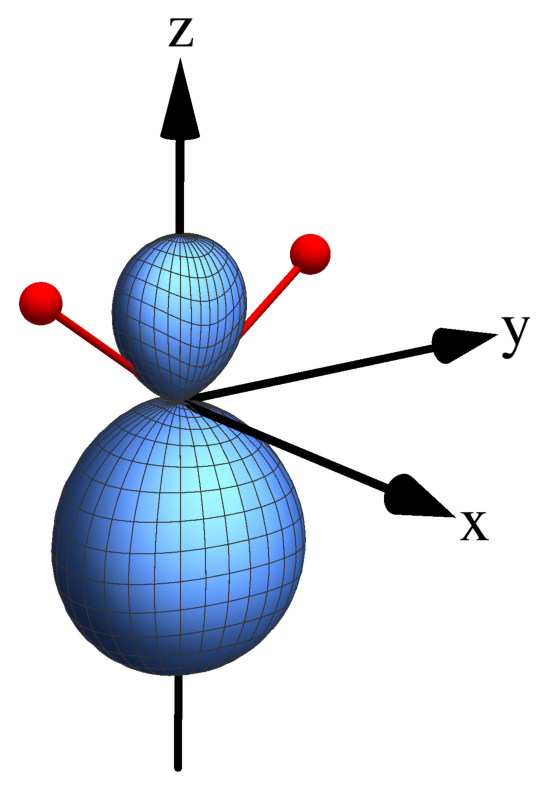
\includegraphics[width=\textwidth]{figures/ch_H2O/3a1/3a1Moccia.eps}
    \caption{Full Moccia $3a_{1}$ orbital}\label{fig:3a1_Moccia}
  \end{subfigure}
  \caption{Schematic display of the $3a_{1}$ molecular orbital (shown
    in blue along the $z$ axis) used to construct
    $V_{\mathrm{eff}}(r,\theta)$. The orbital obtained from a reduced
    expansion in \textsc{sto}s is shown in~(\ref{fig:3a1_reduced}),
    and the complete Moccia orbital is shown
    in~(\ref{fig:3a1_Moccia}). Also indicated (in red in the $y-z$
    plane) is the location of the protons. The $\hat{z}-$axis is the
    direction along which the external electric field of strength
    $F_{0}$ is applied.}
  \label{fig:3a1_prob_density}
\end{figure}

In order to illustrate the fraction of the full Moccia expansion that
our reduced wavefunction~(\ref{eq:3a1Moccia_expansion}) represents,
the projections of the probability densities over the $x-y$ plane are
shown as contours of constant density in
Figure~\ref{fig:3a1_xycontours}, for the height where the protons are
located. From the complete Moccia representation of the $3a_{1}$
\textsc{mo} (in dashed lines), one observes that the location of the
protons (shown as red circles) has an influence on the shape of the
upper lobe in the probability density, i.e., it introduces dependence
on the azimuthal angle $\varphi$. In our simplified expansion, where
only $l=0,1$ and $m=0$ symmetrical parts were included (shown with
solid lines), the probability density misses to represent the proper
azimuthal dependence that follows from the $m\neq 0$ parts.

\begin{figure}
  \centering
  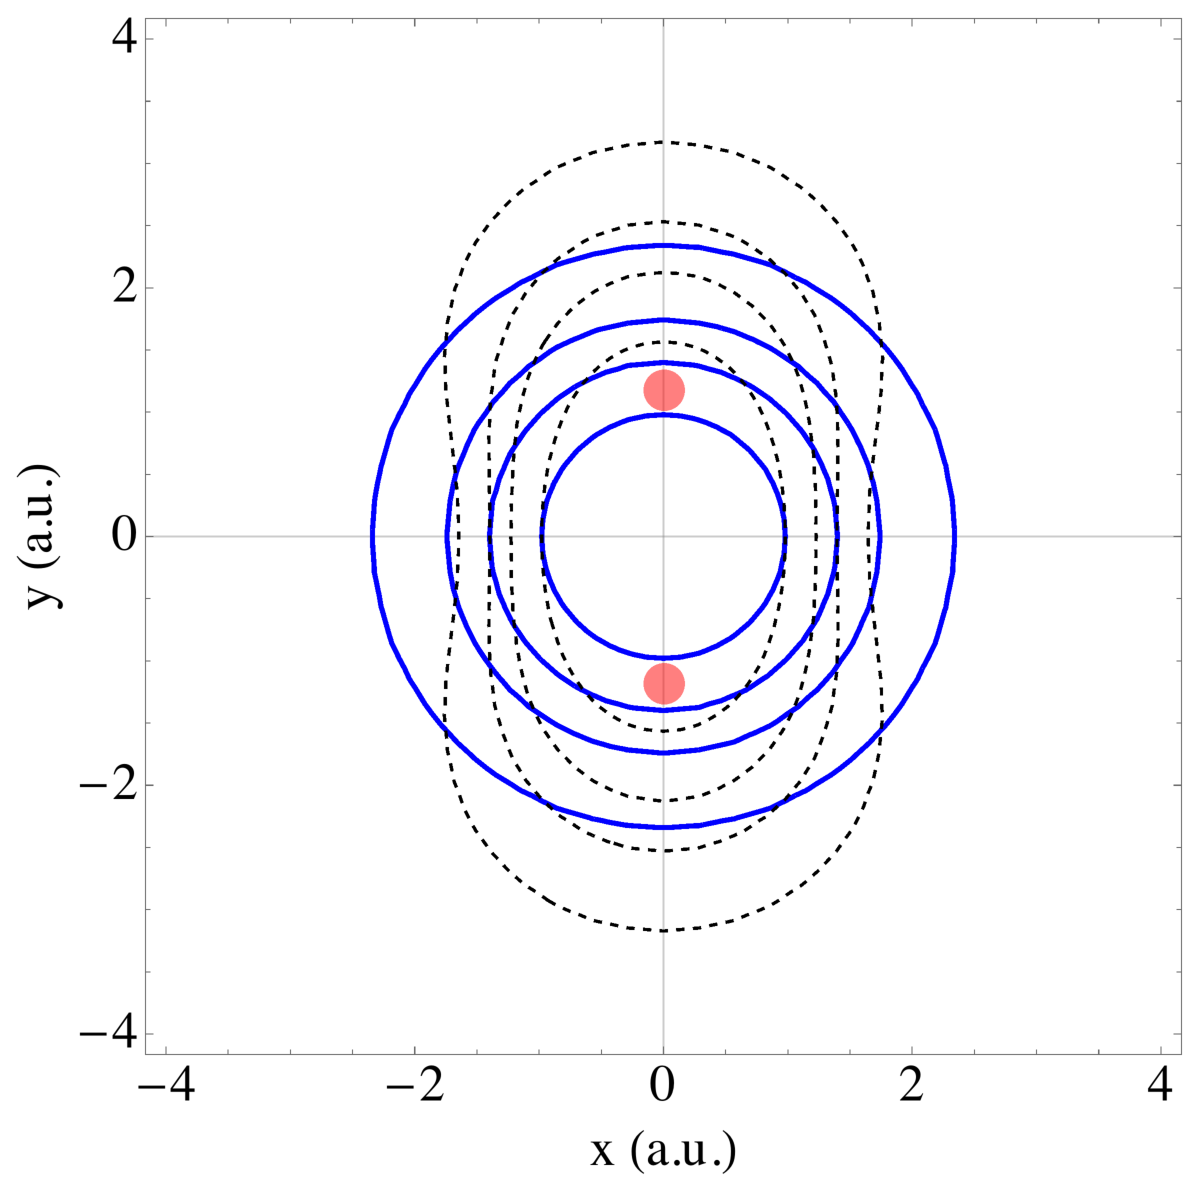
\includegraphics[width=0.6\textwidth]{figures/ch_H2O/3a1/orbitals3a1.eps}
  \caption{Projections of the probability densities for the $3a_{1}$
    orbital on the $x-y$ plane. The simplified \textsc{sto} expansion
    is indicated as continuous blue lines, and the full Moccia
    expansion is indicated as black dashed lines. The protons are also
    indicated as red circles. The chosen contour values are $0.5, 0.3,
    0.2, 0.1$ starting from the innermost contour.}
  \label{fig:3a1_xycontours}
\end{figure}

The non-spherical effective potential corresponding to the
\textsc{sto} expansion~(\ref{eq:3a1Moccia_expansion}),
$V_{\mathrm{eff}}(r,\theta)$, is obtained from the Schr\"{o}dinger
equation in spherical polar coordinates,
%
\begin{eqnarray}
  \left[ -\frac{1}{2} \nabla^{2} +
  V_{\rm{eff}}(r,\theta) \right] \psi_{3a_{1}}(r,\theta) =
  E_{3a_{1}} \psi_{3a_{1}}(r,\theta).
\label{eq:sch_eq3d}
\end{eqnarray}
%
For given $E_{3a_{1}}$ and $\psi_{3a_{1}}(r,\theta)$ it is
straightforward to solve~(\ref{eq:sch_eq3d}) for
$V_{\mathrm{eff}}(r,\theta)$. In order to use this potential to define
a Hamiltonian for the $3a_{1}$ orbital in an electric field, an
asymptotic Latter correction needs to be applied.

Other strategies for finding an effective potential could be pursued,
such as using a density functional, inserting the Moccia wavefunction,
and then performing an azimuthal angle average. Ultimately, one would
like to extend density functional theory~(\textsc{dft}) from finding
ground-state energies to obtaining resonance positions and
widths. This might be feasible using a combination of time-dependent
\textsc{dft} and Floquet theory. The goal of the present work is more
modest: we calculate the response of an isolated molecular orbital in
a simple approximation. Recently, the problem of small molecules in a
dc field has revealed the effect of electron-electron interactions on
Stark resonance parameters~\cite{ScrinziJPhysB_ECS}. It will be
interesting to observe such effects for the water molecule in future
work.


\subsection{Interpolation and Latter correction of the
  non-spherical effective potential}
\label{ch:3a1_Latter}

The non-central effective potential, $V_{\mathrm{eff}}(r,\theta)$,
leads no longer to an orbital of $(l,m)$ symmetry, i.e.,
$2p_{z}$. This reflects the geometry of the problem as a consequence
of the location of the protons. The use of this more general potential
implies that the Latter criterion~\cite{LatterCor_1955}, which ensures
the proper asymptotic behaviour of the potential, is not as
straightforward to implement as in the case of the spherical potential
discussed in Sec.~\ref{ch:1b1_1b2}, where the correction applies
beyond a determined $r$ value~\cite{sarias_2016}. In this case, the
correction must be implemented in the $r-\theta$ plane, by defining a
$\theta-$dependent boundary beyond which the potential obtained
from~(\ref{eq:sch_eq3d}) rises above $-1/r$ in the asymptotic
region~\cite{sarias_2017}.

The $\theta$ coordinate is fixed at two extreme positions, such as
$\theta = 0$ and $\theta = \pi$, in order to find the corresponding
$r$ values $r_{0}$ and $r_{\pi}$, for which
$V_{\mathrm{eff}}(r,\theta) = -1/r$ is satisfied, then we interpolate
between them by introducing the $\theta-$dependent function
%
\begin{eqnarray}
r_{\rm{match}}(\theta) & = & \bar{r} - (r_{\pi} - \bar{r}) \cos\theta,
\label{eq:rMatch}
\end{eqnarray}
%
where $\bar{r} = (r_{0} + r_{\pi})/2$. With this approach we redefine
the effective potential to be the non-central potential derived from
the reduced Moccia wavefunction using Equation~(\ref{eq:sch_eq3d})
when $r < r_{\mathrm{match}}(\theta)$, and $-1/r$ otherwise.

The weighted functions used to construct the Moccia
orbitals~\cite{Moccia_1964} imply a potential difficulty in our
problem. Since these functions are not exact solutions of the
Schr\"{o}dinger equation but were obtained from the variational
principle by implementing a self-consistent
calculation~\cite{Moccia_JCP_2164}, there may be regions in the
$(r,\theta)$ domain where $\psi_{3a_{1}}(r,\theta)$ vanishes, whereas
its second derivative remains finite; this produces a nodal line in
the electronic potential. Thus finding a potential for which our
approximate wavefunction satisfies a Schr\"{o}dinger equations
represents an intricate problem.

It turns out that the nodal region is so narrow that when solving the
Schr\"{o}dinger equation the kinetic energy term dominates and it is
possible to obtain a solution that remains close to that obtained by
the \textsc{hf} method~\cite{Moccia_1964}, regardless of the fact that
there is a region where the effective potential might diverge.

The probability density exhibits two humps indicating the positions of
the protons, which is consistent with
Figure~\ref{fig:3a1_prob_density}, and the effects of the mixing with
the $s-$state. One may argue that one of the reasons this nodal region
in the potential does not have a negative impact on the results is due
to the way the $3a_{1}$ orbital responds to the effective potential by
avoiding this region, its probability density being distributed as
shown in Figure~\ref{fig:density_contours}. A numerical interpolation
of $V_{\mathrm{eff}}(r,\theta)$ is implemented in order to ensure it
continues smoothly over this problematic region.

\begin{figure}
  \centering
  \begin{subfigure}[b]{0.245\linewidth}
    \centering
    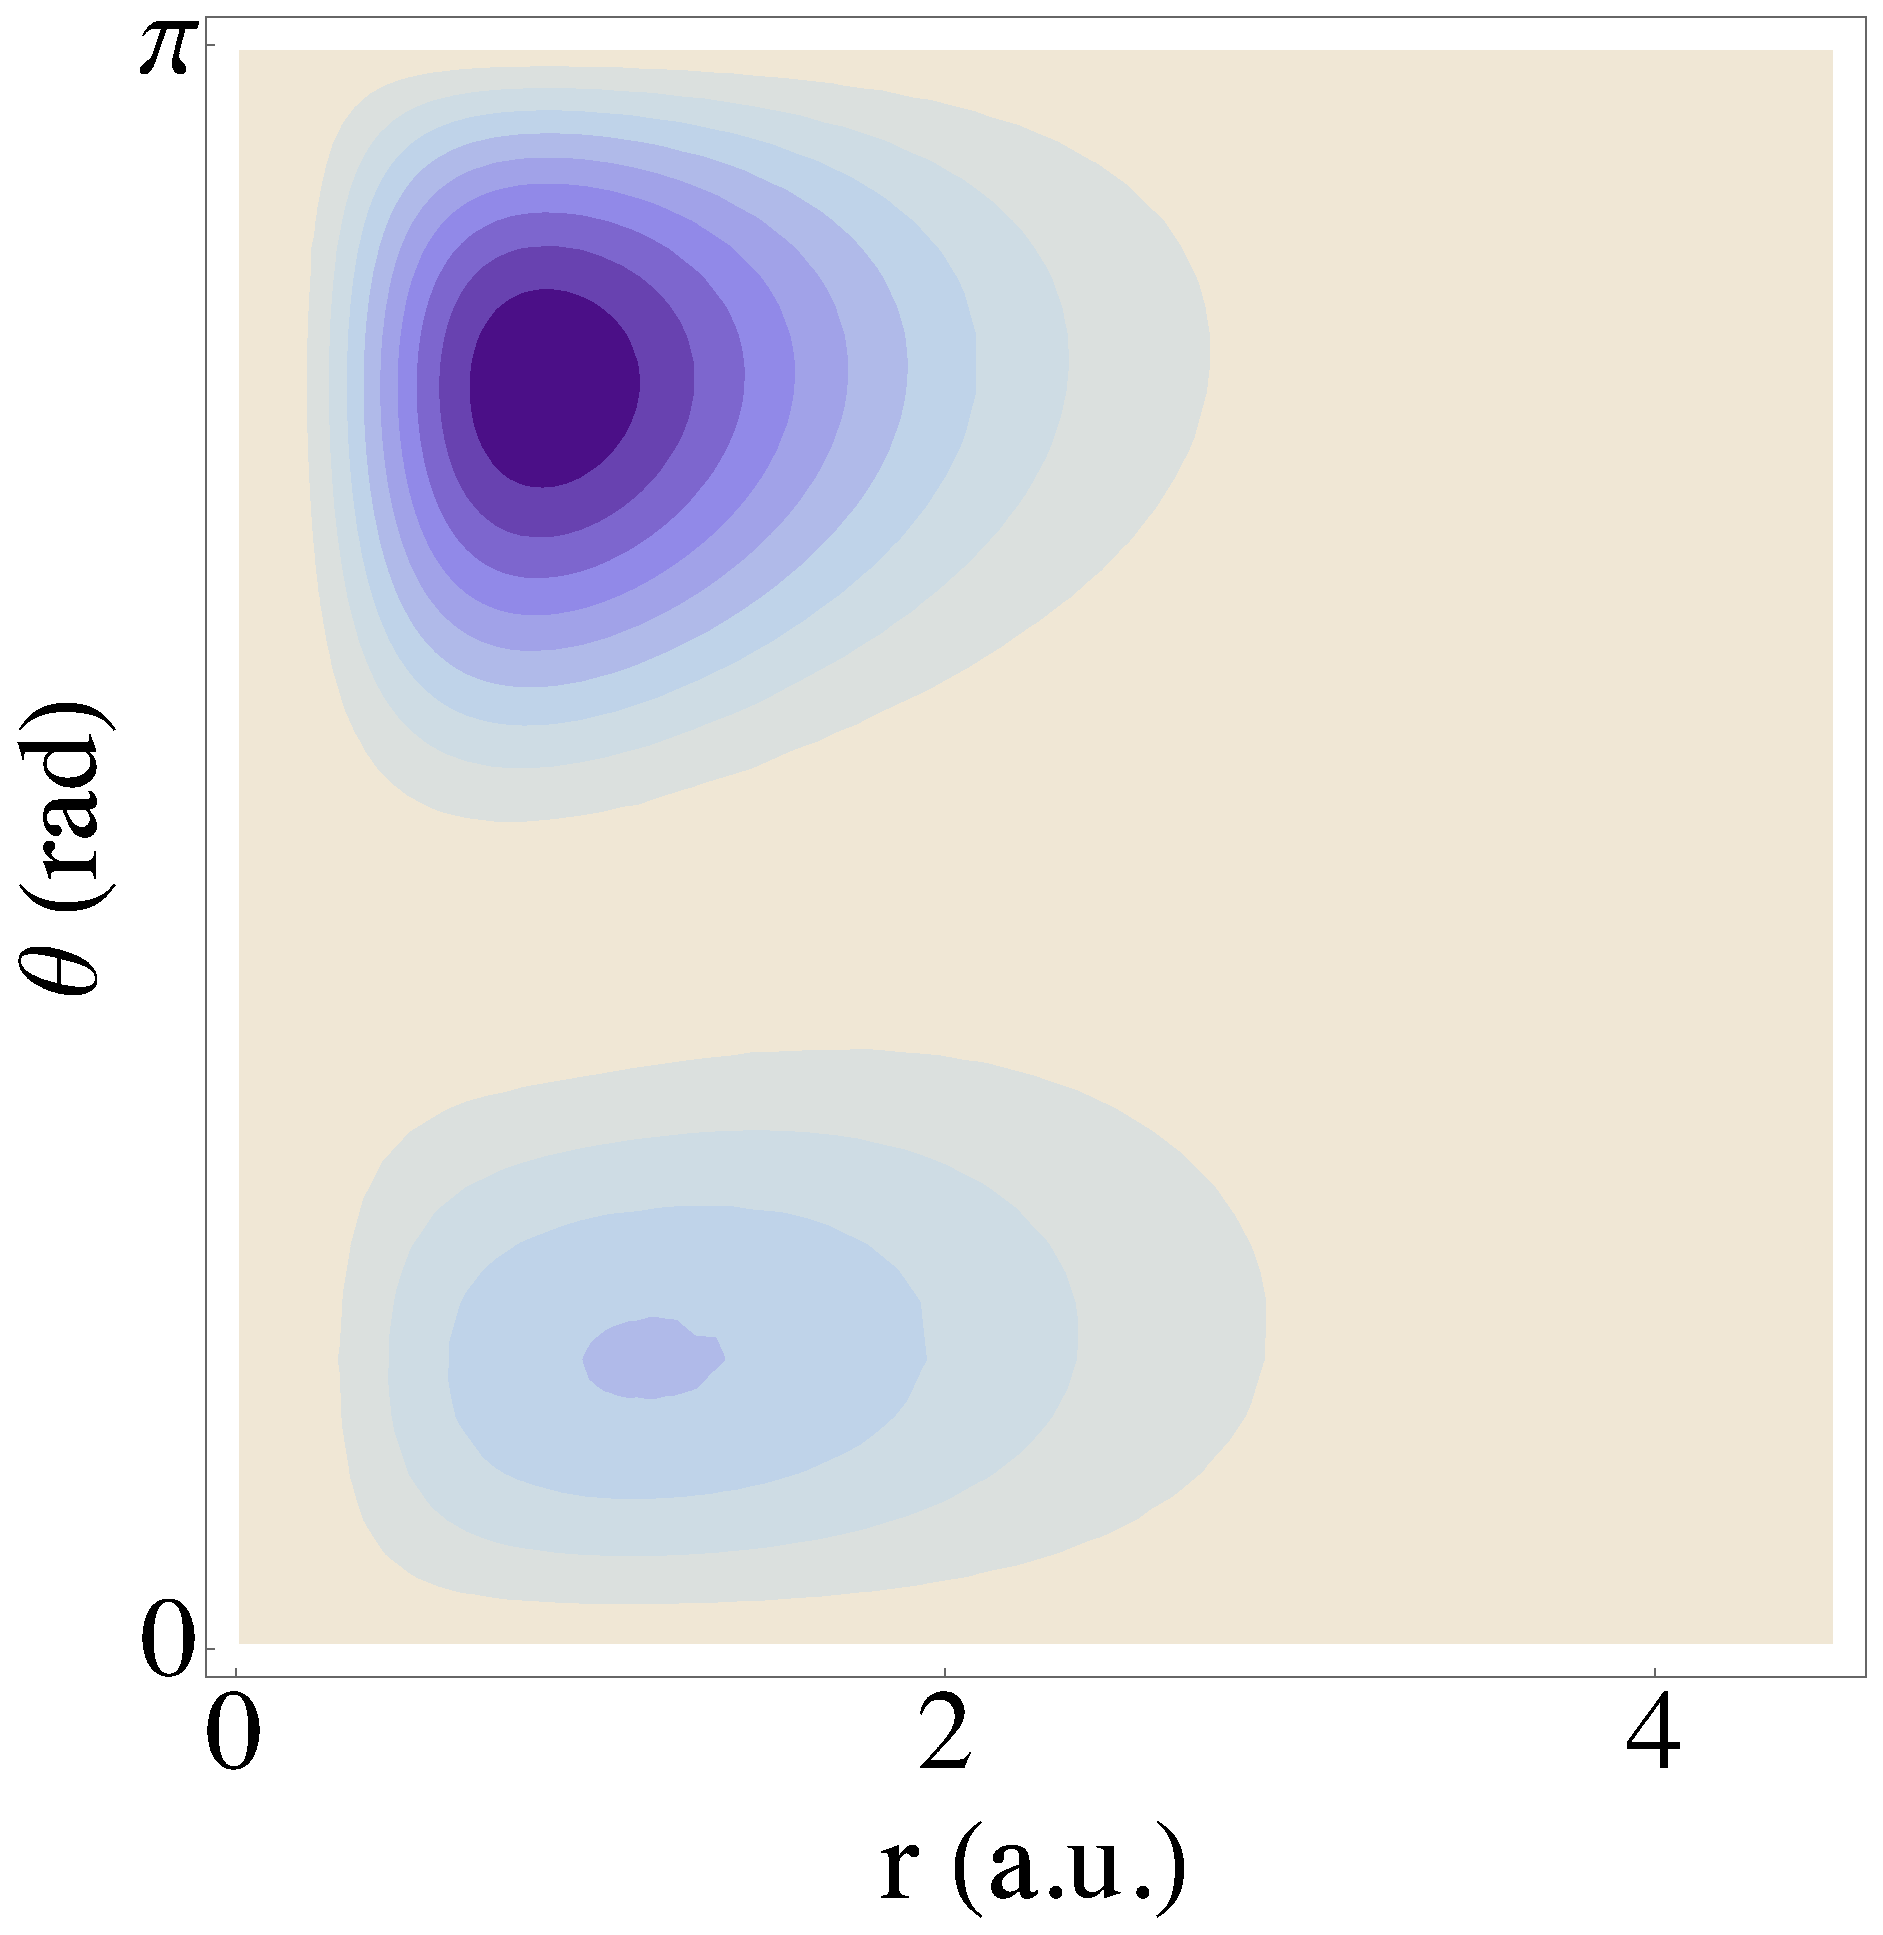
\includegraphics[width=\textwidth]{figures/ch_H2O/3a1/contour3a132s.eps}
    \caption{}\label{fig:Moccia32s}
  \end{subfigure}
  \,
  \begin{subfigure}[b]{0.275\linewidth}
    \centering
    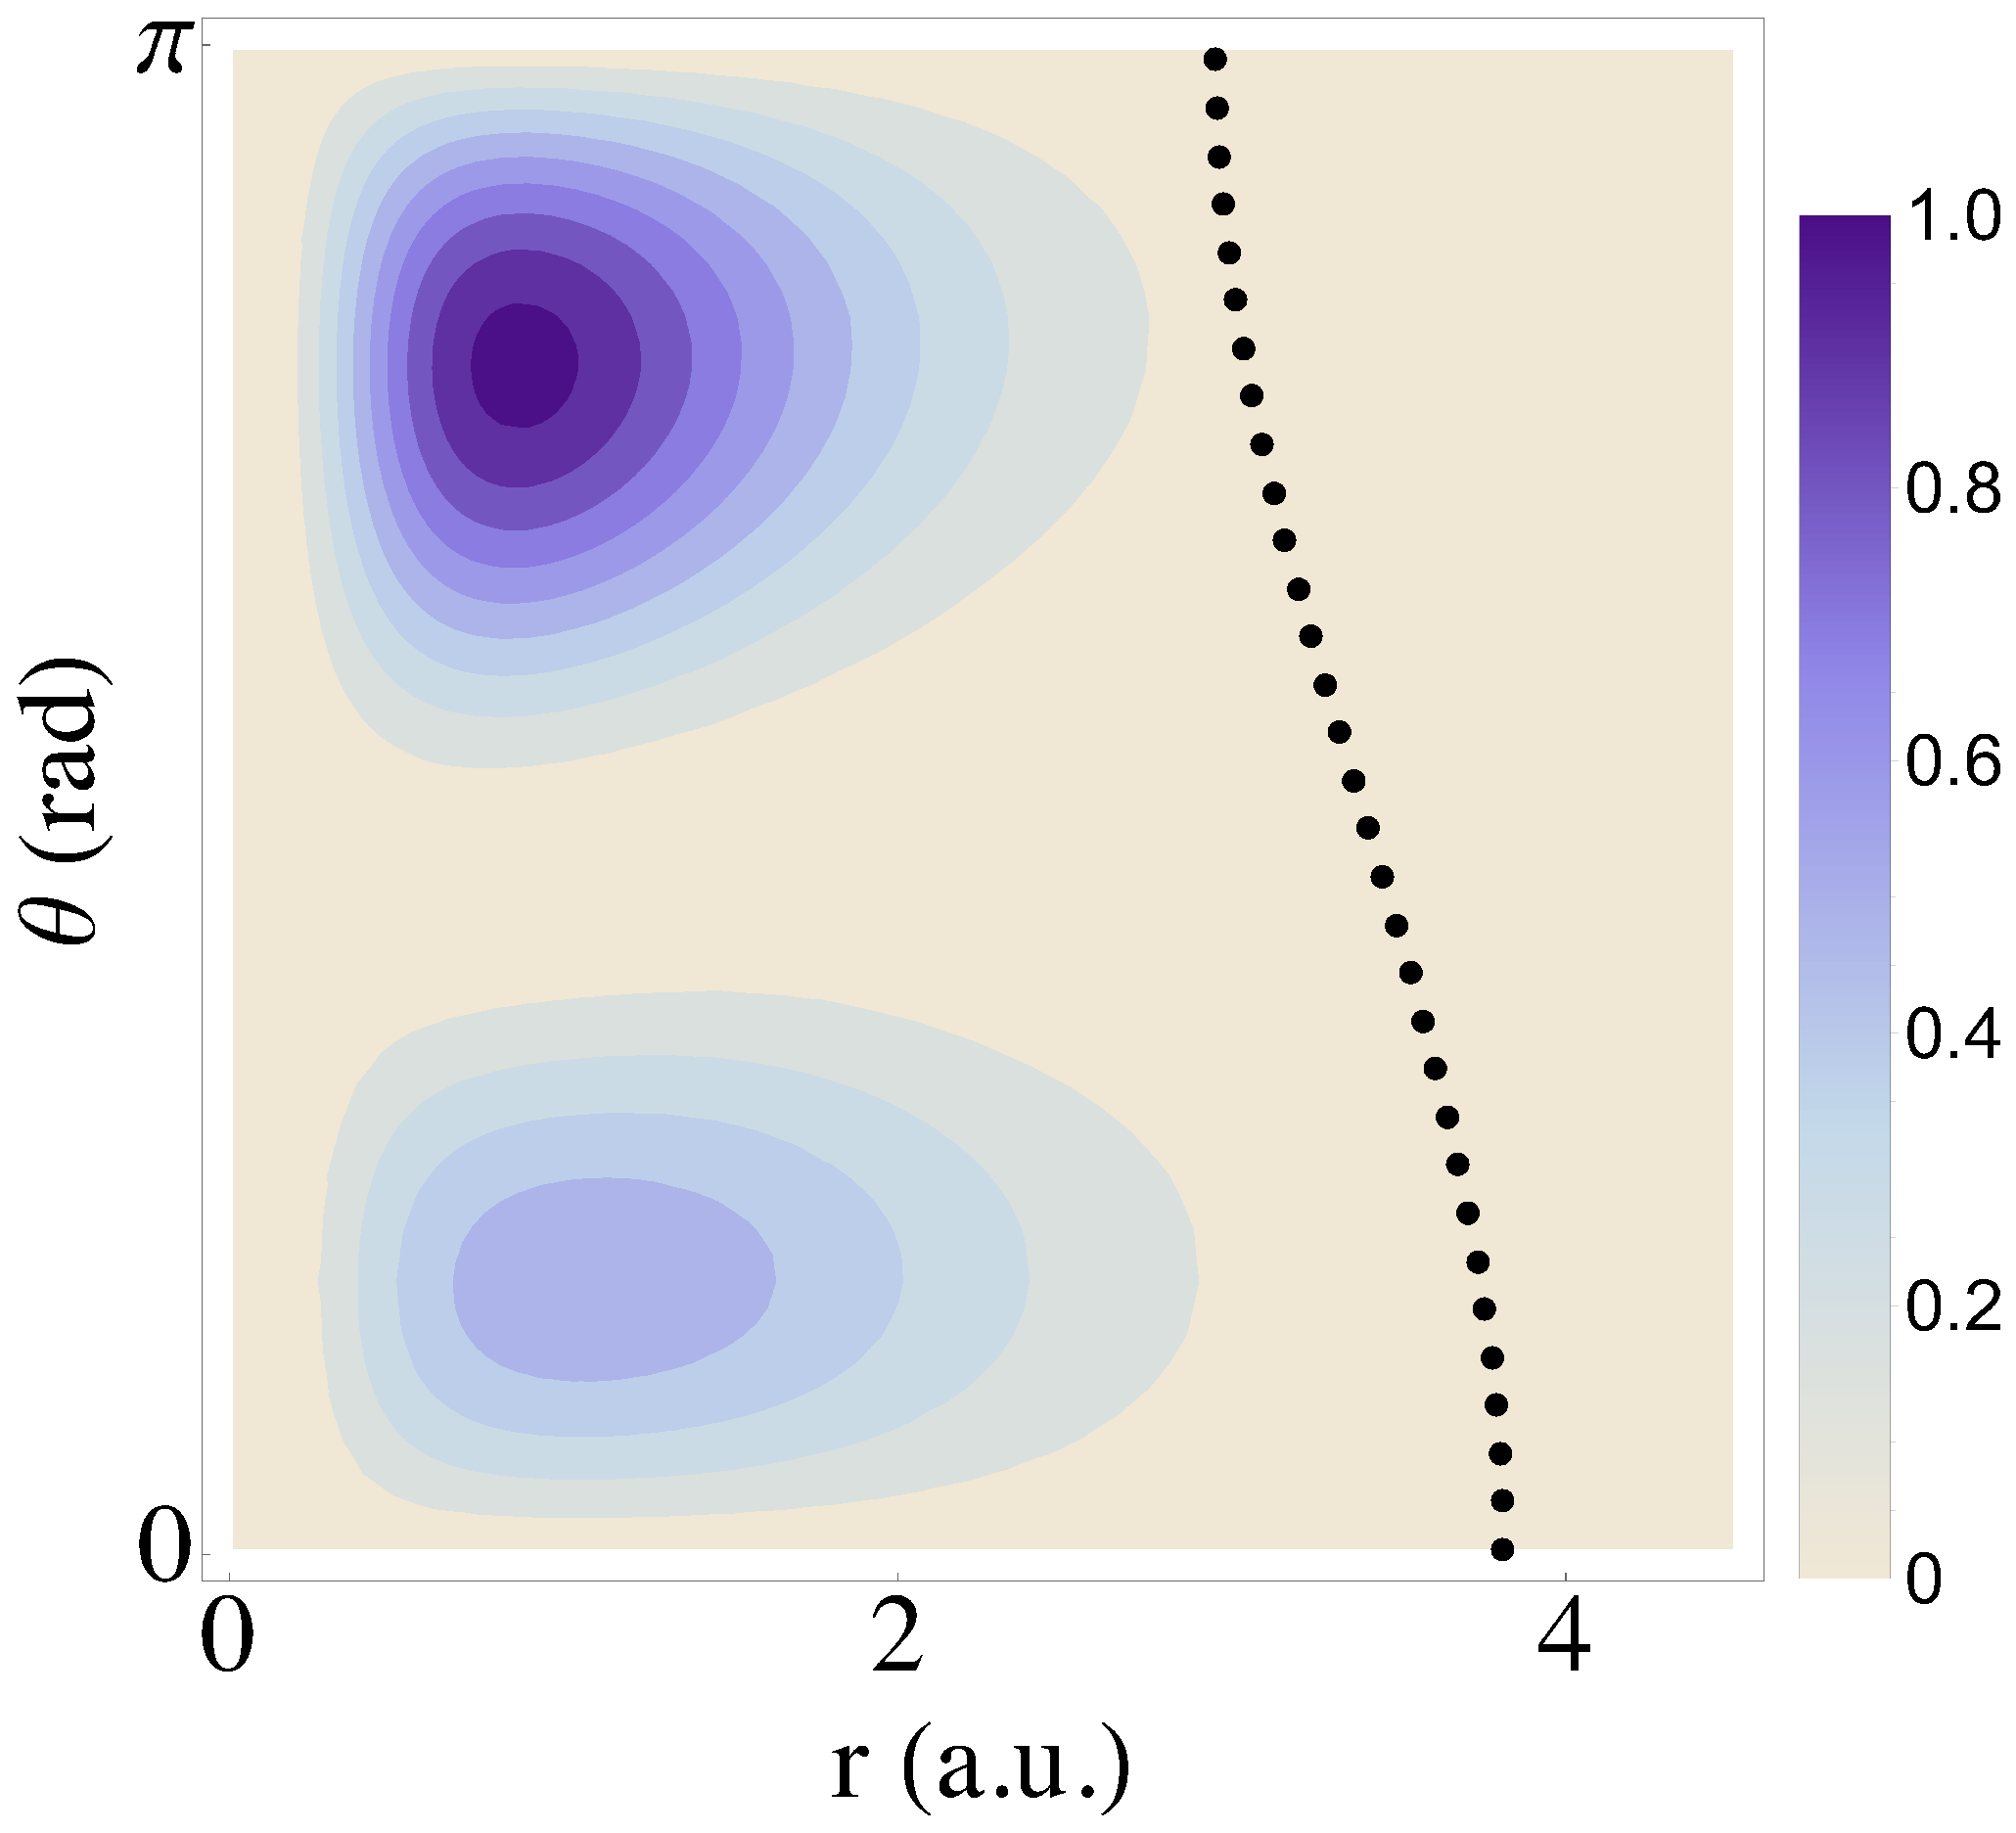
\includegraphics[width=\textwidth]{figures/ch_H2O/3a1/contour3a1intpl.eps}
    \caption{}\label{fig:intp32s}
  \end{subfigure}
  \caption{Contour plots of the scaled probability density,
    $|\psi_{\mathrm{3a_{1}}}|^{2}r^{2}\sin(\theta)/(2\pi)$, for the
    $3a_{1}$ molecular orbital. The orbital density constructed from
    the reduced \textsc{sto} expansion is shown
    in~(\ref{fig:Moccia32s}), while the solution obtained from the
    non-spherical $V_{\mathrm{eff}}(r,\theta)$ with Latter correction
    is shown in~(\ref{fig:intp32s}) along with a dotted line
    indicating where the Latter correction acts. Starting from the
    innermost contours the contour values are $0.45\dots 0.05$ for the
    upper density lobes and $0.2\dots 0.05$ for the lower density
    lobes, in steps of $0.05$.}
  \label{fig:density_contours}
\end{figure}

The interpolation is achieved by collecting data from the evaluation
of the potential on two sections of the $(r,\theta)$ grid in the
vicinity of the nodal line, where the potential evaluates to finite
values. Then, a numerical interpolation was carried out between those
regions in order to obtain a continuous function,
$V_{\mathrm{eff}}^{\mathrm{intp}}(r,\theta)$, on the two-dimensional
grid. The Latter correction is applied to the interpolated potential
and the effective potential is defined according to~(\ref{eq:rMatch}):
%
\begin{eqnarray}
  V_{\mathrm{eff}}(r,\theta) = \left\{
  \begin{split}
    V_{\mathrm{eff}}^{\mathrm{intp}}(r,\theta)\
    & \mathrm{~for} & r < r_{\mathrm{match}}(\theta) \\
    -1/r\ & \mathrm{~for} &  r > r_{\mathrm{match}}(\theta)
  \end{split}
\right.
\label{eq:latterVeff}
\end{eqnarray}
%

Figure~\ref{fig:Moccia32s} shows the probability density for the
$3a_{1}$ \textsc{mo} as a contour plot in the $r-\theta$ plane as
obtained from the reduced Moccia expansion in
\textsc{sto}s~(\ref{eq:3a1Moccia_expansion}). Figure~\ref{fig:intp32s}
shows the same for the solution of the Schr\"{o}dinger
equation~(\ref{eq:sch_eq3d}) using the interpolated
$V_{\mathrm{eff}}(r,\theta)$, defined in
Equation~(\ref{eq:latterVeff}), with the Latter
correction~\cite{LatterCor_1955} applied in the asymptotic $r-$region.

The effective potential~(\ref{eq:latterVeff}) results in the
probability density shown in Figure~\ref{fig:intp32s} and yields an
orbital energy of $-0.5579\ \mathrm{a.u.}$ for the $3a_{1}$
\textsc{mo}, with a relative change of $0.32\%$ in comparison with the
self-consistent result of Moccia~\cite{Moccia_1964} of
$-0.5561\ \mathrm{a.u.}$.

As Figure~\ref{fig:intp32s} indicates, the implementation of the
Latter correction to the orbital-dependent potential obtained from
Equation~(\ref{eq:sch_eq3d}) introduces a slight re-adjustment of the
density, with a somewhat higher probability density in the region $0 <
\theta < \pi/2$. The probabilities for finding the electron at $\pi/2
< \theta < \pi$ is $66.2\%$ before the Latter correction is applied
(Figure~\ref{fig:Moccia32s}) and becomes $63.5\%$ for the case shown
in Figure~\ref{fig:intp32s}.

\subsection{Exterior complex scaling}
\label{ch:3a1_ecs}

For our aim of computing the resonance parameters that describe the
tunneling process, a modified exterior complex scaling to the radial
coordinates was implemented. As was described in
Sec.~\ref{ch:ecs_1b11b2}, the $r-$coordinate is extended into the
complex plane by the phase function $\chi(r)$,
Eq.~(\ref{eq:ecs_theta}), with $r$ replaced by $r^{*} =
r\exp[i\chi(r)]$. The phase function $\chi(r)$ is chosen to be very
small for $r$ values smaller than the Latter radius $\bar{r}$. It then
turns on from nearly zero to reach an asymptotic value
$\chi_{\mathrm{s}}$ at $r-$values just outside where the Latter
correction is applied, i.e., $r_{\mathrm{s}} > r_{\mathrm{match}}$. In
such a way as to provide exterior complex scaling without a hard
radius at which a derivative discontinuity would have to be
applied~\cite{ecsScrinzi}.

A non-Hermitian Hamiltonian results from considering the additional
terms that the modified complex scaling to the radial coordinates
introduces in the Schr\"{o}dinger equation. The complex wavefunction
is separated into real and imaginary parts, $\psi_{R(I)}$, such that
the problem of describing the ionization regime of the $3a_{1}$
\textsc{mo} under an external dc field applied along the orientation
axis of the orbital is expressed in terms of a system of partial
differential equations for the real and imaginary parts of
$\widetilde{\psi}(r,\theta)$ in spherical polar coordinates given
explicitly as Eq.~(\ref{eq:pde_system}). Schematically, the equations
are extensions of the field-free Schr\"{o}dinger
equation~(\ref{eq:sch_eq3d}) and $\widetilde{\psi}(r,\theta)$
satisfies~\cite{sarias_2017}
%
\begin{eqnarray}
  \begin{split}
    \left[ -\frac{1}{2}\nabla^{2} + V_{\mathrm{eff}}(r,\theta)
      \pm F_{0}z \right] \widetilde{\psi} = (E_{R} - i\Gamma/2)
    \widetilde{\psi},
  \end{split}
  \label{eq:sch_tunneling_params}
\end{eqnarray}
%
where $E_{R}$ is the resonance position and $\Gamma$ the
width. Compared to Eq.~(\ref{eq:sch_eq3d}), the Hamiltonian in
Eq.~(\ref{eq:sch_tunneling_params}) contains the interaction with the
external field and complex scaling is responsible for the replacement
$E_{3a_{1}} \to E_{R} - i\Gamma/2$; while $\widetilde{\psi}$ remains
square integrable.

The domains of $r$ and $\theta$ values are restricted to the intervals
$r\in[\epsilon, r_{\mathrm{max}}]$ and $\theta\in[\eta,\pi-\eta]$,
with typical values $\epsilon = 10^{-2}\ \mathrm{a.u.}$, $\eta =
10^{-2}$, $r_{\mathrm{max}} = 28\ \mathrm{a.u.}$ In the limit of low
field strengths, i.e., $F_{0} = 0.05, 0.06$, the value of
$r_{\mathrm{max}}$ was increased to $40\ \mathrm{a.u.}$ in order to
ensure the outer turning points lie inside the grid, as the tunneling
barrier extends to larger $r$.

The problem of finding a solution of the Schr\"{o}dinger equation for
the $3a_{1}$ \textsc{mo} with contributions of $2s$ and $2p-$type
states requires a set of boundary conditions that describes the
properties of the orbital on the grid. In contrast with the $m = \pm
1$ solutions obtained for the $1b_{1}$ and $1b_{2}$ \textsc{mo}s of
H$_{2}$O~\cite{sarias_2016}, Neumann boundary conditions are
implemented for the angular coordinate $\theta$ in order to obtain an
eigenstate and orbital energy consistent with the variational
results~\cite{Moccia_1964}. This choice of boundary conditions, that
the derivative with respect to $\theta$ vanishes at the limits of the
mesh $(\theta = 0 ~\mathrm{and}~ \theta = \pi)$, leads to solutions
$\psi_{R(I)}(r,\theta)$ with a probability density consistent with the
$\theta-$dependence of the $3a_{1}$ orbital, as shown in
Figure~\ref{fig:density_contours}.

% NEXT SECTION
%The physical parameters of interest, namely the resonance position,
%$E_{R}$, and width, $\Gamma = -2E_{I}$, that characterize the
%tunneling process of the quasi-stationary state when an external
%electric dc field is applied along the $\pm\hat{z}$ directions, were
%found by solving the system of partial differential equations
%(Ref.~\cite{PhysRevA.94.053413}) for a set of field strength values,
%$F_{0}$, as if it were an inhomogeneous problem. In the vicinity of a
%location in the $(r,\theta)$ plane where the probability amplitude is
%expected to be large, a two-parameter root search was implemented to
%determine $\{E_{R},E_{I}\}$, the complex energy that maximizes the
%probability density amplitude in the $2d-$grid.

\section{Stark resonance parameters}
\label{ch:stark_params}

In the following subsections we present plots of the physical
parameters of interest, namely the resonance position, $E_{R}$, and
width, $\Gamma = -2E_{I}$, that characterize the tunneling process of
the quasi-stationary state when an external electric dc field is
applied along the $\pm\hat{z}$ directions. The system of partial
differential equations~(\ref{eq:pde_system}) is solved for a set of
field strength values, $F_{0}$, as if it were an inhomogeneous
problem. In the vicinity of a location in the $(r,\theta)$ plane in
which the probability amplitude is expected to be large, a
two-parameter root search is implemented in order to determine
${E_{R}, E_{I}}$, the complex energy that maximizes the probability
density amplitude in the $2d-$grid.


\subsection{$1b_{1}$ and $1b_{2}$ molecular orbitals}
\label{ch:1b1_1b2_results}

% include the plots that the first 3 paragraphs in secIII(PRA2016)
% refer to about the systematic studies of the relevant parameters for
% the calculation

\begin{figure}
  \centering
  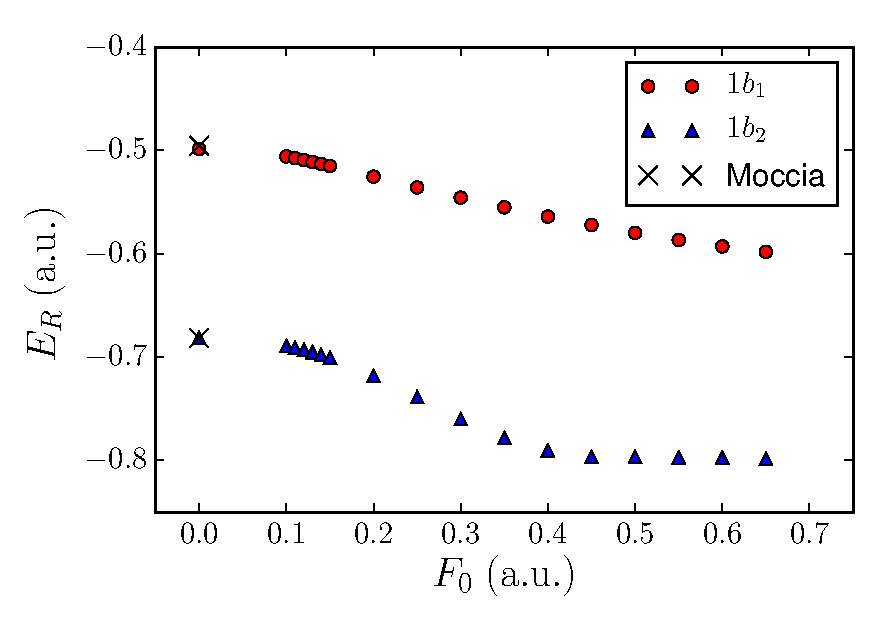
\includegraphics[width=0.7\textwidth]{figures/ch_H2O/1b1_1b2/resPositionvsF1b11b2.eps}
  \caption{Resonance position as a function of the external field
    strength $F_{0}$ for the $1b_{1}$ (red circles) and $1b_{2}$ (blue
    triangles) \textsc{mo}s of H$_{2}$O.}
  \label{fig:1b11b2_position}
\end{figure}

\begin{figure}
  \centering
  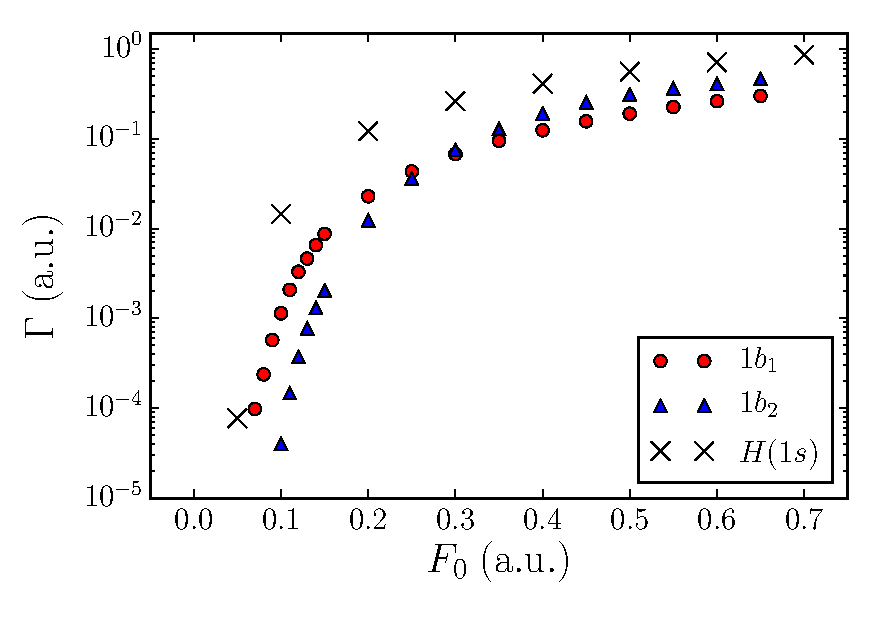
\includegraphics[width=0.7\textwidth]{figures/ch_H2O/1b1_1b2/resWidthvsF1b11b2H1s.eps}
  \caption{Resonance width as a function of the external field
    strength $F_{0}$ for the $1b_{1}$ (red circles) and $1b_{2}$ (blue
    triangles) \textsc{mo}s of H$_{2}$O. For comparison, atomic
    hydrogen H$(1s)$ ionization rates from
    Refs.~\cite{Telnov_1989,Kolosov_1987} are shown as crosses.}
  \label{fig:1b11b2_width}
\end{figure}

Figure~\ref{fig:1b11b2_position} shows the resonance position $E_{R}$
as obtained from the present calculations for the weakly bound
$1b_{1}$ and the strongly bound $1b_{2}$ valence orbitals as a
function of applied electric field strength $F_{0}$. In the limit of
zero field the calculation reproduces the \textsc{scf} eigenvalues of
Moccia~\cite{Moccia_1964}. The field has to be strong (in comparison
with atomic hydrogen results for $2p$ orbitals~\cite{Telnov_1989}) in
order to change the resonance position appreciably. For the more
deeply bound $1b_{2}$ orbital the shift in resonance position
saturates with field strength.

In Figure~\ref{fig:1b11b2_width} the resonance widths are shown for
both orbitals as functions of external field strength $F_{0}$. The
graphs display threshold behavior at the weaker field strengths. As
expected, we find a lower threshold (critical field strength) for the
more weakly bound $1b_{1}$ orbital. Interestingly, however, at a field
strength of about $F_{0} = 0.3\ \mathrm{a.u.}$ the values for the
widths cross; that is, the deeper bound $1b_{2}$ orbital displays a
larger ionization rate as the field strength is increased further.

Also shown in Figure~\ref{fig:1b11b2_width} are the widths for the
H($1s$) orbital from Refs.~\cite{Telnov_1989,Kolosov_1987}. They can
be compared to the $1b_{1}$ orbital results, since the binding energy
is very close in the free-field limit. Since the tunneling barrier is
mostly in the asymptotic regime where the potential energy has a
$-1/r$ tail, it is not surprising that the widths for
H$_{2}$O($1b_{1}$) and H($1s$) share some similarity in shape. In the
tunneling region H($1s$) has an ionization rate that is larger by
about an order of magnitude. In the over-barrier regime, however, the
ionization rates come to within a factor of 3. Reasons for why the
$1b_1$ water molecular orbital is harder to ionize than H($1s$) have
to do with the different shape of the orbital density ($m=1$ \emph{vs}
the spherical H($1s$) density), and the substantially more attractive
potential at shorter distances.

An examination of contour plots of the densities $\Psi^{*}\Psi$, as
well as of the potential energies $V_{\mathrm{eff}} - F_{0}z$ for
different field strengths (both as a function of $r,\theta$), allows
us to make the following observations. For field strengths $F_{0} <
0.1\ \mathrm{a.u.}$ there is a barrier the electrons need to penetrate
in order to be ionized. From the potential-energy plot shown in
Figure~\ref{fig:1b11b2_position} one can see that for weak fields
(small values of $F_{0}$) the barrier is longer for the more deeply
bound $1b_{2}$ orbital. This explains why the ionization threshold
occurs for $F_{0} > 0.1\ \mathrm{a.u.}$ for this orbital, which is
about a factor of $2$ larger than for the $1b_{1}$ orbital.

The field-strength region where the ionization rates (resonance
widths) display a change in character, i.e., turn over to rise much
more gradually with the field strength $F_{0}$, can be characterized
as a regime where there is a narrow potential saddle at small $\theta$
in the vicinity of $r \approx 3\ \mathrm{a.u.}$, such that electron
flux can leave and is then accelerated by the electric field. The
crossing of the ionization rates for the $1b_{1}$ and $1b_{2}$
orbitals occurs since the saddle in the potential becomes effectively
lower at strong fields for the $1b_{2}$ orbital. This can be inferred
from the comparison of the two effective potentials, which share the
same asymptotic behaviour beyond $r = 4.3\ \mathrm{a.u.}$ (see
Figure~\ref{fig:Veff1b11b2}).

The origin for the different radial dependencies of the effective
potential for the two orbitals can be found in the geometry of the
water molecule. The weakly bound $1b_{1}$ orbital has its lobes
perpendicular to the plane defined by the location of the three
nuclei. Therefore, it is least affected by the two protons. The
$1b_{2}$ orbital explores the potentials due to the protons more
strongly in the \textsc{scf} calculation of Moccia, and therefore, the
resulting $V_{\mathrm{eff}}(r)$ has a more attractive region in the
range $0.7\ \mathrm{a.u.} < r < 4.3\ \mathrm{a.u.}$.

%The numerical results are summarized in Table~\ref{tab:1b11b2_results}
%for further reference, i.e., for future comparisons with calculations
%based on other models for the molecular orbitals.

%\begin{table}[t]
%\centering
%\caption{\label{tab:1b11b2_results} Resonance positions and widths for
%  different field strengths (in atomic units). The numbers in
%  parentheses indicate the exponent $k$; that is, the numbers are to
%  be multiplied by $10^{k}$.}
%\begin{tabular}{rrrrr}
%\toprule
% & & $1b_{1}$ & & $1b_{2}$ \\
%$F_{0}$ & $E_{R}$ & $\Gamma$ & $E_{R}$ & $\Gamma$ \\
%\midrule
%$0.1$ & $-0.506$ & $1.14(-3)$ & $-0.689$ & $4.04(-5)$ \\
%$0.2$ & $-0.525$ & $2.28(-2)$ & $-0.718$ & $1.23(-2)$ \\
%$0.3$ & $-0.546$ & $6.74(-2)$ & $-0.760$ & $7.51(-2)$ \\
%$0.4$ & $-0.564$ & $1.24(-1)$ & $-0.790$ & $1.91(-1)$ \\
%$0.5$ & $-0.580$ & $1.90(-1)$ & $-0.796$ & $3.11(-1)$ \\
%$0.6$ & $-0.593$ & $2.61(-1)$ & $-0.797$ & $4.11(-1)$ \\
%\bottomrule
%\end{tabular}
%\end{table}


\subsection{$3a_{1}$ molecular orbital}
\label{ch:3a1_results}

The numerical results from applying the procedure described in
Section~\ref{ch:3a1} are shown in Figures~\ref{fig:3a1_position}
and~\ref{fig:3a1_width}.

\begin{figure}
  \centering
  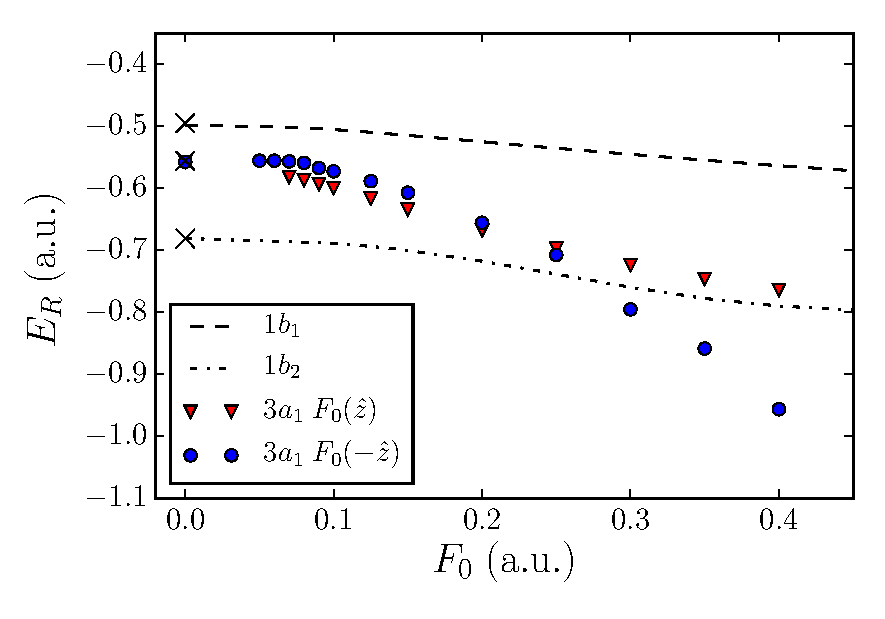
\includegraphics[width=0.7\textwidth]{figures/ch_H2O/3a1/resPosvsForbitals_compf32snew.eps}
  \caption{Resonance position in atomic units as a function of the
    external field strength $F_{0}$ and the orientation of the field,
    along the $\pm\hat{z}$ direction (red triangles/blue circles), for
    the $3a_{1}$ \textsc{mo} of H$_{2}$O. As a reference, the resonance
    position values for the $1b_{1}$ (dashed line) and $1b_{2}$
    (dot-dashed line) \textsc{mo}s are also included.}
  \label{fig:3a1_position}
\end{figure}

\begin{figure}
  \centering
  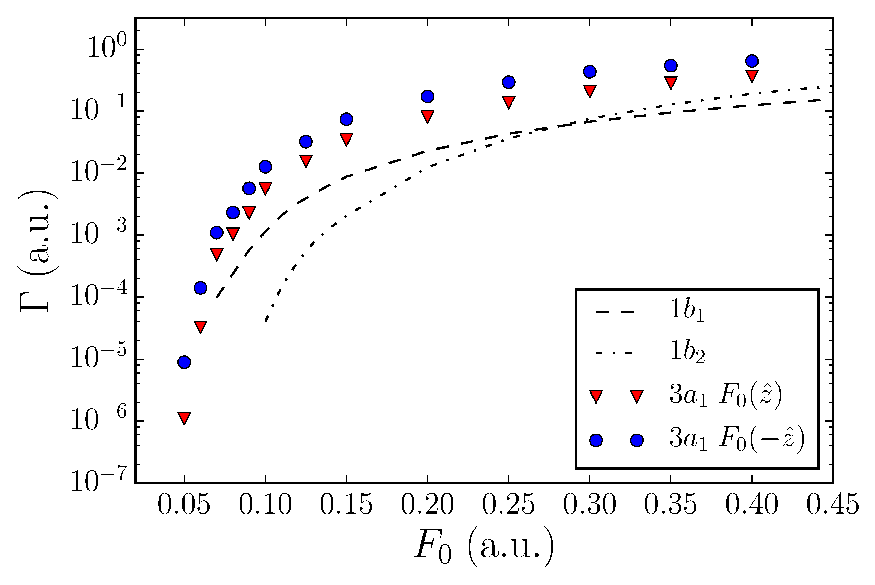
\includegraphics[width=0.7\textwidth]{figures/ch_H2O/3a1/resWidthvsForbitals_compf32snew.eps}
  \caption{Resonance width in atomic units as a function of the
    external field strength $F_{0}$ and the orientation of the field,
    along the $\pm\hat{z}$ direction (red triangles/blue circles), for
    the $3a_{1}$ \textsc{mo} of H$_{2}$O. For reference, the resonance
    widths for the $1b_{1}$ (dashed line) and $1b_{2}$ (dot-dashed
    line) \textsc{mo}s are also shown.}
  \label{fig:3a1_width}
\end{figure}

The resonance positions $E_{R}$ are shown in
Figure~\ref{fig:3a1_position} for external fields applied along the
$\pm\hat{z}$ directions (red triangles/blue circles) for a range of
external field strengths. For reference, the resonance positions
obtained for the $1b_{1}$ and $1b_{2}$ \textsc{mo}s using a
spherically symmetric potential, $V_{\mathrm{eff}}(r)$, are also
indicated in the form of dashed and dot-dashed lines respectively. For
zero field strength $F_{0} = 0$ self-consistent eigenenergies obtained
by Moccia~\cite{Moccia_1964} are included as black crosses for the
three valence orbitals of interest. As expected, the resonance
position for the $3a_{1}$ orbital is bracketed by those for the
$1b_{1}$ and $1b_{2}$ orbitals.

It can be noticed that for external fields applied along the
$-\hat{z}$ direction, where most of the density is located, the field
strength $F_{0}$ has to be strong, i.e., $F_{0}>0.1\ \mathrm{a.u.}$,
for the resonance position to change appreciably. On the other hand,
the resonance position for fields applied along $+\hat{z}$ appears to
be more sensitive at weaker fields. However the barrier appears to be
longer for external fields applied along the $+\hat{z}$ direction, at
a field strength of about $F_{0} = 0.2\ \mathrm{a.u.}$ the position
values cross, indicating a higher sensitivity of the resonance
positions for fields applied along the negative $\hat{z}$ direction as
the field strength is increased further.

Figure~\ref{fig:3a1_width} shows the resonance widths corresponding to
external fields applied along the $\pm\hat{z}$ directions, as a
function of the field strength $F_{0}$. The results obtained with a
symmetric effective potential, $V_{\mathrm{eff}}(r)$, for the $1b_{1}$
and $1b_{2}$ \textsc{mo}s are also shown as dashed and dot-dashed
lines for comparison purposes.

In analogy to the $m=\pm 1$ orbitals, the ionization rates for the
$3a_{1}$ \textsc{mo}, associated with the lifetime of the decaying
state via $\Gamma\tau=1$, exhibit a threshold behaviour at the weaker
field strengths. Interestingly, for the two directions of the applied
field, we find a lower critical field strength for the $3a_{1}$
orbital in comparison to what the more weakly bound orbital, $1b_{1}$,
indicates.  In the tunneling region, the $3a_{1}$ orbital for fields
applied along the $-\hat{z}$ direction (blue squares) shows an
ionization rate that is about one order of magnitude larger than the
ionization rate for fields applied in the opposite direction (red
triangles), this gap becomes narrower as the field strength increases
toward the over-barrier regime.

The numerical results for the H$_{2}$O valence orbitals studied in
this chapter, $1b_{1}$, $1b_{2}$ and $3a_{1}$, are summarized in
Table~\ref{tab:3a1_results} for further reference, i.e., to allow
comparison with future calculations based on other models for the
molecular orbitals.


\begin{table}[t]
\centering
\caption{\label{tab:3a1_results} Resonance positions and widths for
  different field strengths (in atomic units). The orientation of the
  external field is indicated by $\pm\hat{z}$. The numbers in
  parentheses indicate the exponent $k$, so that the numbers are
  multiplied by $10^{k}$.}
\begin{tabular}{rrrrrrrrr}
\toprule
&& $3a_{1}(\hat{z})$ && $3a_{1}(-\hat{z})$ && $1b_{1}$ && $1b_{2}$ \\
\midrule
$F_{0}$&$E_{R}$&$\Gamma$&$E_{R}$&$\Gamma$&$E_{R}$&$\Gamma$&$E_{R}$&$\Gamma$ \\
\midrule
$0.05$ &   --~~ &$1.09(-6)$&$-0.556$&$8.91(-6)$ & --~~ & --~~ & --~~ & --~~ \\
$0.06$ &   --~~ &$3.23(-5)$&$-0.556$&$1.41(-4)$ & --~~ & --~~ & --~~ & --~~ \\
$0.07$ &$-0.582$&$4.82(-4)$&$-0.557$&$1.09(-3)$&$-0.502$&$9.82(-5)$ & --~~ & --~~ \\
$0.08$ &$-0.587$&$1.03(-3)$&$-0.559$&$2.31(-3)$&$-0.503$&$2.38(-4)$ & --~~ & --~~ \\
$0.09$ &$-0.594$&$2.26(-3)$&$-0.568$&$5.65(-3)$&$-0.504$&$5.72(-4)$ & --~~ & --~~ \\
$0.1$  &$-0.600$&$5.53(-3)$&$-0.573$&$1.26(-2)$&$-0.506$&$1.14(-3)$&$-0.689$&$4.04(-5)$\\
$0.125$&$-0.617$&$1.54(-2)$&$-0.589$&$3.21(-2)$&$-0.510$&$3.76(-3)$&$-0.694$&$5.45(-4)$\\
$0.15$ &$-0.635$&$3.41(-2)$&$-0.607$&$7.39(-2)$&$-0.515$&$8.73(-3)$&$-0.701$&$2.04(-3)$\\
$0.2$  &$-0.668$&$7.98(-2)$&$-0.656$&$1.72(-1)$&$-0.525$&$2.28(-2)$&$-0.718$&$1.23(-2)$\\
$0.25$ &$-0.698$&$1.37(-1)$&$-0.708$&$2.92(-1)$&$-0.536$&$4.33(-2)$&$-0.739$&$3.61(-2)$\\
$0.3$  &$-0.724$&$2.07(-1)$&$-0.796$&$4.31(-1)$&$-0.546$&$6.74(-2)$&$-0.760$&$7.51(-2)$\\
$0.35$ &$-0.747$&$2.81(-1)$&$-0.859$&$5.40(-1)$&$-0.555$&$9.46(-2)$&$-0.778$&$1.27(-1)$\\
$0.4$  &$-0.765$&$3.60(-1)$&$-0.957$&$6.40(-1)$&$-0.564$&$1.24(-1)$&$-0.790$&$1.91(-1)$\\
\bottomrule
\end{tabular}
\end{table}



%%% Local Variables:
%%% mode: latex
%%% TeX-master: "thesis"
%%% End:
